% 这是中国科学院大学计算机科学与技术专业《计算机体系结构(研讨课)》使用的实验报告 Latex 模板
% 本模板与 2024 年 2 月 Jun-xiong Ji 完成, 更改自由 Shing-Ho Lin 和 Jun-Xiong Ji 于 2022 年 9 月共同完成的基础物理实验模板
% 如有任何问题, 请联系: jijunxoing21@mails.ucas.ac.cn
% This is the LaTeX template for report of Experiment of Computer Organization and Design courses, based on its provided Word template. 
% This template is completed on Febrary 2024, based on the joint collabration of Shing-Ho Lin and Junxiong Ji in September 2022. 
% Adding numerous pictures and equations leads to unsatisfying experience in Word. Therefore LaTeX is better. 
% Feel free to contact me via: jijunxoing21@mails.ucas.ac.cn

\documentclass[11pt]{article}

\usepackage[a4paper]{geometry}
\geometry{left=2.0cm,right=2.0cm,top=2.5cm,bottom=2.5cm}

\usepackage{ctex} % 支持中文的LaTeX宏包
\usepackage{amsmath,amsfonts,graphicx,subfigure,amssymb,bm,amsthm,mathrsfs,mathtools,breqn} % 数学公式和符号的宏包集合
\usepackage{algorithm,algorithmicx} % 算法和伪代码
\usepackage[noend]{algpseudocode} % 算法和伪代码
\usepackage{fancyhdr} % 自定义页眉页脚
\usepackage[framemethod=TikZ]{mdframed} % 创建带边框的框架
\usepackage{fontspec} % 字体设置
\usepackage{adjustbox} % 调整盒子大小
\usepackage{fontsize} % 设置字体大小
\usepackage{tikz,xcolor} % 绘制图形和使用颜色
\usepackage{multicol} % 多栏排版
\usepackage{multirow} % 表格中合并单元格
\usepackage{pdfpages} % 插入PDF文件
\usepackage{listings} % 在文档中插入源代码
\usepackage{wrapfig} % 文字绕排图片
\usepackage{bigstrut,multirow,rotating} % 支持在表格中使用特殊命令
\usepackage{booktabs} % 创建美观的表格
\usepackage{circuitikz} % 绘制电路图
\usepackage{zhnumber} % 中文序号(用于标题)
\usepackage{tabularx} % 表格折行

\definecolor{dkgreen}{rgb}{0,0.6,0}
\definecolor{gray}{rgb}{0.5,0.5,0.5}
\definecolor{mauve}{rgb}{0.58,0,0.82}
\lstset{
  frame=tb,
  aboveskip=3mm,
  belowskip=3mm,
  showstringspaces=false,
  columns=flexible,
  framerule=1pt,
  rulecolor=\color{gray!35},
  backgroundcolor=\color{gray!5},
  basicstyle={\small\ttfamily},
  numbers=none,
  numberstyle=\tiny\color{gray},
  keywordstyle=\color{blue},
  commentstyle=\color{dkgreen},
  stringstyle=\color{mauve},
  breaklines=true,
  breakatwhitespace=true,
  tabsize=3,
}

% 轻松引用, 可以用\cref{}指令直接引用, 自动加前缀. 
% 例: 图片label为fig:1
% \cref{fig:1} => Figure.1
% \ref{fig:1}  => 1
\usepackage[capitalize]{cleveref}
% \crefname{section}{Sec.}{Secs.}
\Crefname{section}{Section}{Sections}
\Crefname{table}{Table}{Tables}
\crefname{table}{Table.}{Tabs.}

% \setmainfont{Palatino Linotype.ttf}
% \setCJKmainfont{SimHei.ttf}
% \setCJKsansfont{Songti.ttf}
% \setCJKmonofont{SimSun.ttf}
\punctstyle{kaiming}
% 偏好的几个字体, 可以根据需要自行加入字体ttf文件并调用

\renewcommand{\emph}[1]{\begin{kaishu}#1\end{kaishu}}

% 对 section 等环境的序号使用中文
\renewcommand \thesection{\zhnum{section}、}
\renewcommand \thesubsection{\arabic{section}}


%%%%%%%%%%%%%%%%%%%%%%%%%%%
%改这里可以修改实验报告表头的信息
\newcommand{\name}{姚永舟}
\newcommand{\studentNum}{2022K8009926016}
\newcommand{\major}{计算机科学与技术}
\newcommand{\labNum}{2}
\newcommand{\labName}{互联网协议实验、流完成时间实验}
%%%%%%%%%%%%%%%%%%%%%%%%%%%

\begin{document}

\begin{center}
  \LARGE \bf 中国科学院大学 \\《计算机体系结构(研讨课)》实验报告
\end{center}

\begin{center}
  \emph{姓名} \underline{\makebox[7em][c]{\name}} 
  % 如果名字比较长, 可以修改box的长度"8em"为其他值
  \emph{学号} \underline{\makebox[12em][c]{\studentNum}}
  \emph{专业} \underline{\makebox[15em][c]{\major}}\\
  \emph{实验项目编号} \underline{\makebox[3em][c]{\labNum}}
  \emph{实验名称} \underline{\makebox[30em][c]{\labName}}\\
\end{center}


  

\begin{center}
  \LARGE \bf 实验一:互联网协议实验
\end{center}

\section{实验内容}

\begin{enumerate}
  \item 在节点h1上开启wireshark抓包,用wget下载www.ucas.ac.cn页面
  
  \item 调研说明wireshark抓到的几种协议ARP, DNS, TCP, HTTP, HTTPS
  
  \item   调研解释h1下载ucas页面的整个过程,几种协议的运行机制
  
\end{enumerate}

\section{实验流程}

\begin{enumerate}
  \item 在终端执行 sudo mn --nat,将host连接至internet, 并启动mininet
  \item 在mininet中输入 xterm h1, 打开控制h1的终端
  \item 在h1中输入 echo "nameserver 1.2.4.8" > /etc/resolv.conf,设置DNS服务器
  \item 在h1中输入 wireshark \& ,打开wireshark
  \item 在wireshark中选择h1-eth0,开始抓包
  \item 在h1中输入 wget www.ucas.ac.cn,下载网页
  \item 观察wireshark抓包结果,并调研分析获得的几种互联网协议
\end{enumerate}
\section{实验结果}

\textbf{ARP协议}

\begin{figure} [htbp]
  \centering
  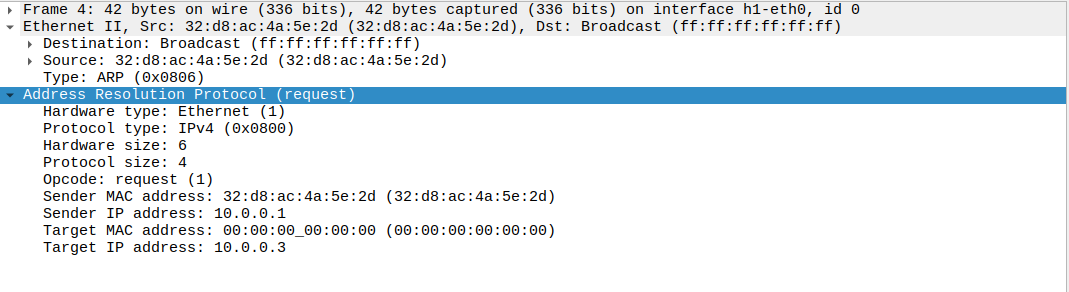
\includegraphics[width=0.8\textwidth]{fig/arp.png}
  \caption{ARP协议}
  \label{fig:ARP}
\end{figure}

\newpage 

\textbf{DNS协议}

\begin{figure} [htbp]
  \centering
  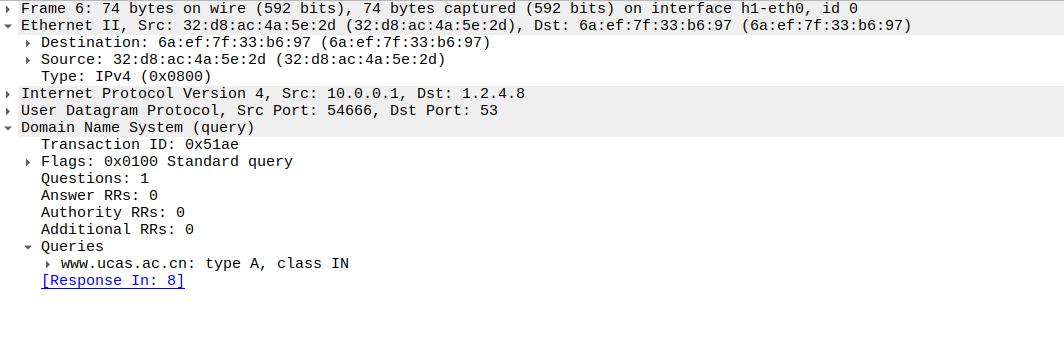
\includegraphics[width=0.8\textwidth]{fig/dns.png}
  \caption{DNS协议}
  \label{fig:DNS}
\end{figure}

 
\textbf{TCP协议}

\begin{figure} [htbp]
  \centering
  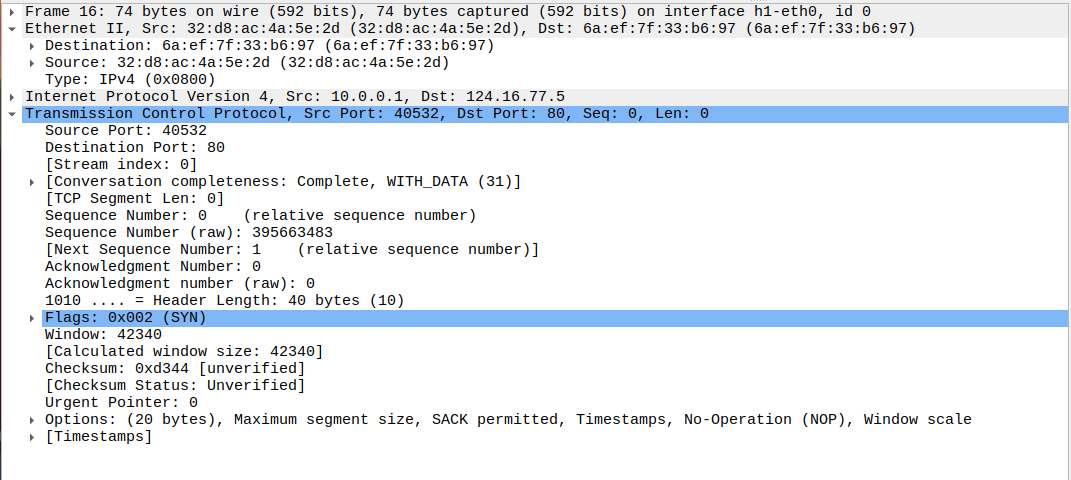
\includegraphics[width=0.8\textwidth]{fig/tcp.png}
  \caption{TCP协议}
  \label{fig:TCP}
\end{figure}

\textbf{HTTP协议}

\begin{figure} [htbp]
  \centering
  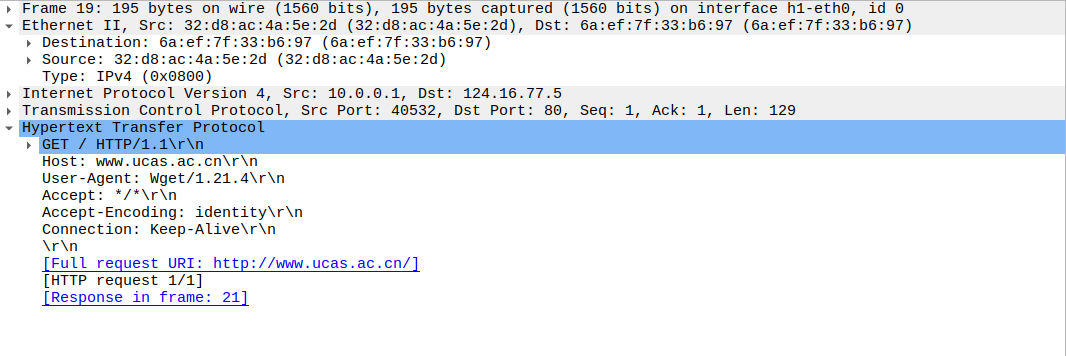
\includegraphics[width=0.7\textwidth]{fig/http.png}
  \caption{HTTP协议}
  \label{fig:HTTP}

\end{figure}

\newpage


\textbf{TCP flow}
\begin{figure}[htbp]
  \centering
  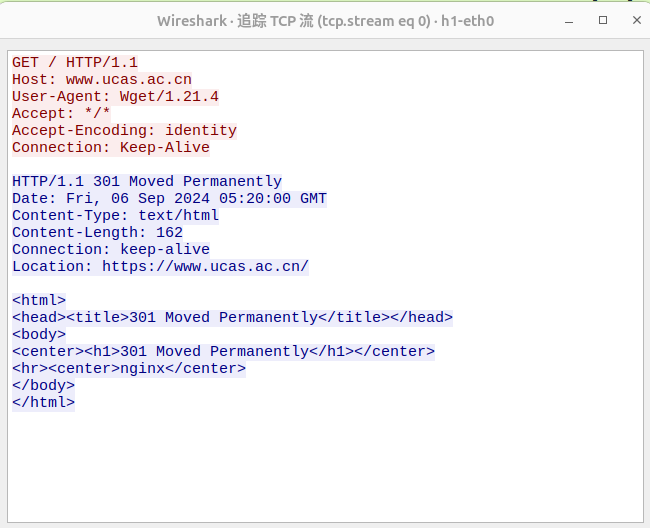
\includegraphics[width=0.8\textwidth]{fig/tcp_flow.png}
  \caption{TCP flow}
  \label{fig:TCP flow}
\end{figure}

\section{实验分析}

在获取UCAS主页的传输过程中使用了以下几种协议:ARP协议、DNS协议、TCP协议、HTTP协议。

并且各个协议的封装层次如下:

\begin{enumerate}
  \item ARP协议:Ethernet < ARP
  \item DNS协议:Ethernet < IP < UDP < DNS
  \item TCP协议:Ethernet < IP < TCP
  \item HTTP协议:Ethernet < IP < TCP < HTTP
\end{enumerate}

\section{调研结果}

\textbf{1. ARP(地址解析)协议}

ARP 协议“Address Resolution Protocol”(地址解析协议)的缩写。其作用是在以太网
环境中,数据的传输所依懒的是MAC 地址而非IP 地址,而将已知IP 地址转换为MAC 地址的
工作是由ARP 协议来完成的。

在局域网中,网络中实际传输的是“帧”,帧里面是有目标主机的MAC 地址的。在以太网
中,一个主机和另一个主机进行直接通信,必须要知道目标主机的MAC 地址。目标MAC 地址
是通过地址解析协议获得的。所谓“地址解析”就是主机在发送帧前将目标IP 地址转换成目
标MAC 地址的过程。ARP 协议的基本功能就是通过目标设备的IP 地址,查询目标设备的
MAC 地址,以保证通信的顺利进行。ARP 通过发送一个ARP 请求帧到局域网中的所有设备来
查找目标设备的MAC 地址。这个请求包含源设备的IP 地址和MAC 地址。目标设备收到请
求后,会回复一个包含其IP 地址和MAC 地址的ARP 响应帧。

\textbf{2. DNS(域名系统)协议}

DNS (Domain Name System)是一个应用层协议,域名系统(DNS)的作用是将人类可读
的域名(如www.exa-
mple.com)转换为机器可读的IP 地址(如192.0.2.44)。 DNS 系统使用
树状层次结构,包括多个DNS 服务器,它们负责不同的域名解析。当用户输入一个域名时,
客户端的DNS 解析器将向根DNS 服务器发送查询,然后逐级查询更低级别的DNS 服务器,
直到找到与域名相关的IP 地址。

DNS 协议建立在UDP 或TCP 协议之上,默认使用53 号端口。客户端默认通过UDP 协
议进行通讯,但是由于广域网中不适合传输过大的UDP 数据包,因此规定当报文长度超过了
512 字节时,应转换为使用TCP 协议进行数据传输。DNS 是一种可以将域名和IP 地址相互映
射的以层次结构分布的数据库系统。

\textbf{3. TCP(传输控制)协议}

TCP (Transmission Control Protocol 传输控制协议)是一种面向连接的、可靠的、基于
字节流的传输层通信协议,由IETF 的RFC 793 定义。在简化的计算机网络OSI 模型中,它完
成第四层传输层所指定的功能。

应用层向TCP 层发送用于网间传输的、用8 位字节表示的数据流,然后TCP 把数据流分
区成适当长度的报文段(通常受该计算机连接的网络的数据链路层的最大传输单元(MTU)的限
制) 。之后TCP 把结果包传给IP 层,由它来通过网络将包传送给接收端实体的TCP 层。TCP
将用户数据打包构成报文段,它发送数据时启动一个定时器,另一端收到数据进行确认,对失序
的数据重新排序,丢弃重复的数据。简单说, TCP 协议的作用是,保证数据通信的完整性和可靠
性,防止丢包。

\textbf{4. HTTP协议}

HTTP 协议(超文本传输协议HyperText Transfer Protocol),它是基于TCP 协议的应用
层传输协议,用于从WWW 服务器传输超文本到本地浏览器的传输协议, HTTP 是一个应用层
协议,由请求和响应构成,是一个标准的客户端和服务器模型,简单来说就是客户端和服务端进
行数据传输的一种规则。它指定了客户端可能发送给服务器什么样的消息以及得到什么样的响
应。客户端发送HTTP 请求到服务器,请求特定资源(如网页或图像)。服务器收到请求后,
会发送HTTP 响应,包含请求的资源以及相关信息。HTTP 通信通常是无状态的,每个请求和
响应都独立于之前的请求和响应。


\textbf{5. h1下载ucas页面的整个过程以及几种协议的运行机制}

1. DNS解析域名www.ucas.ac.cn,获取IP地址

2. 三次握手建立TCP连接

  第一次握手:客户端发送SYN包至服务器,并进入SYN_SENT状态,等待服务器确认


  \begin{figure}[htbp]
    \centering
    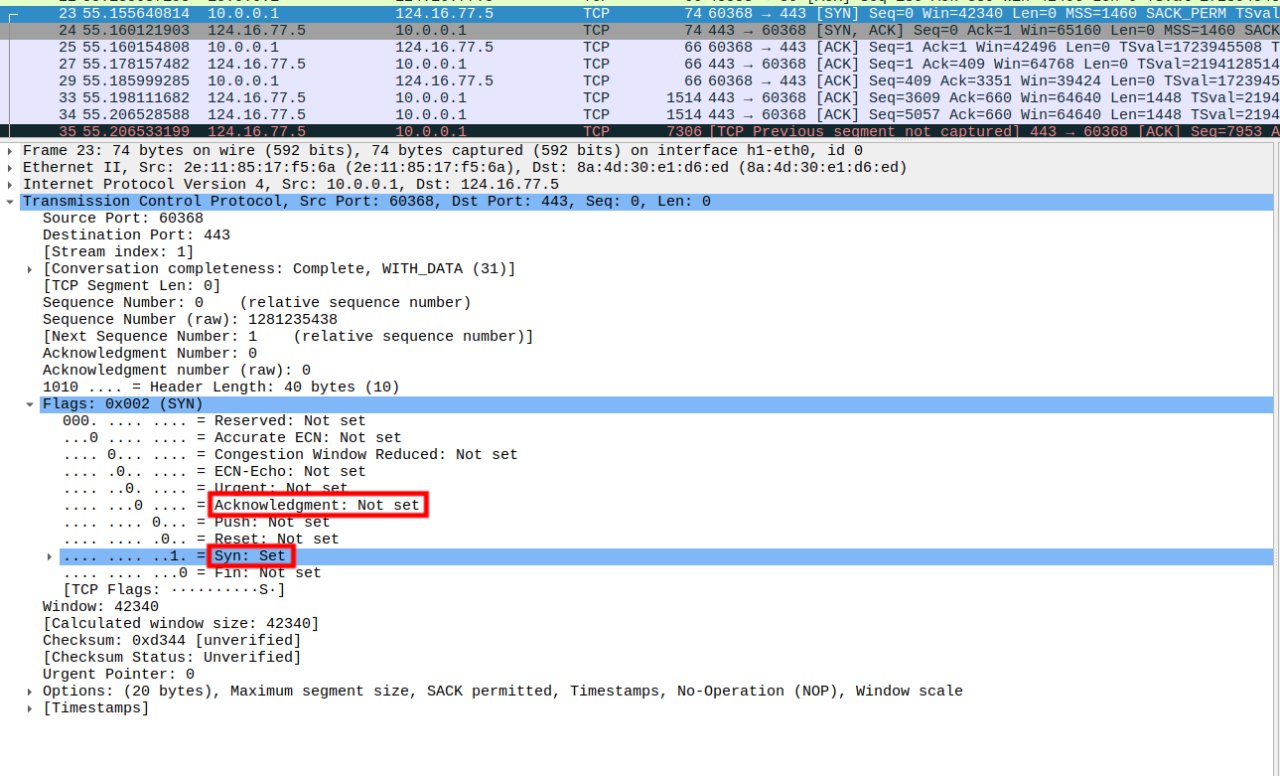
\includegraphics[width=0.7\textwidth]{fig/hand1.png}
    \caption{第一次握手}
    \label{fig:1}
  \end{figure}

  第二次握手:服务器收到客户端的SYN包,发送一个ACK,同时发送自己的SYN,此时服务器进入SYN_RCVD状态
  \begin{figure}[htbp]
    \centering
    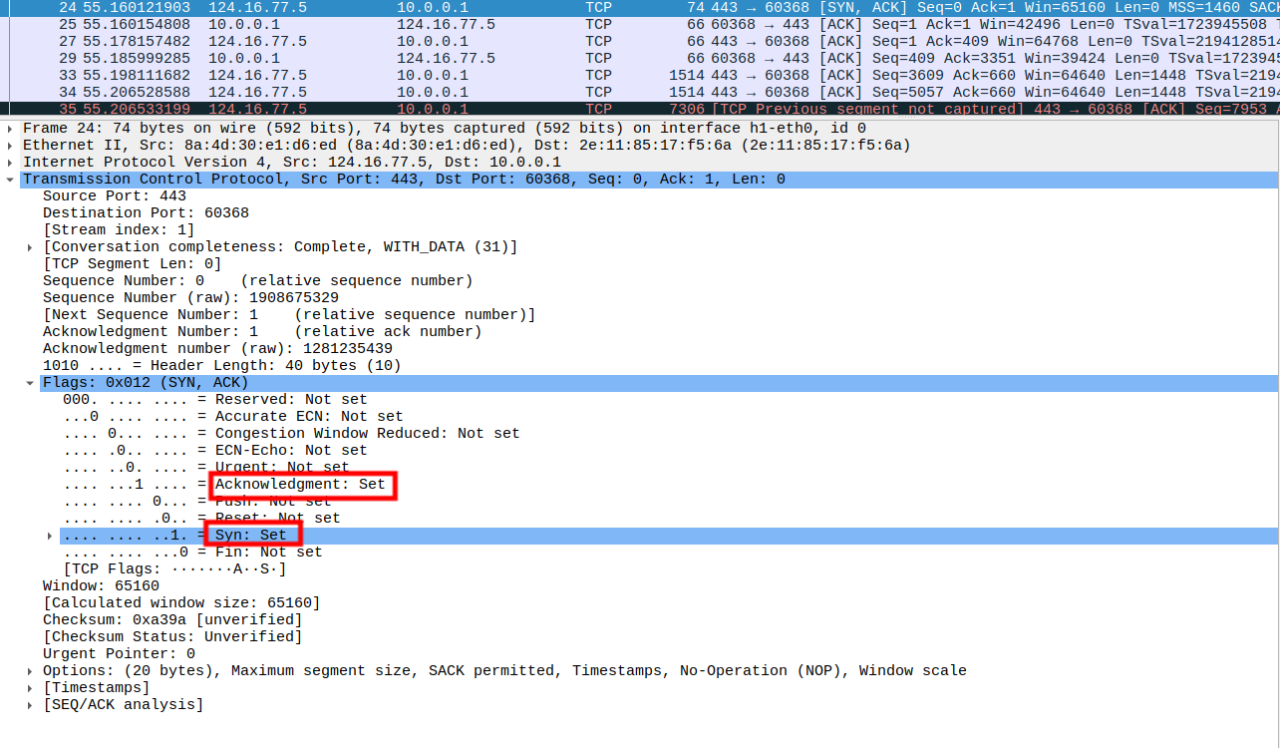
\includegraphics[width=0.8\textwidth]{fig/hand2.png}
    \caption{第二次握手}
    \label{fig:2}
  \end{figure}


  第三次握手:客户端接收到服务器发送的SYN+ACK后,进入ESTABLISHED状态,并发送服务器SYN包的确认ACK,服务器接收到客户端ACK后,进入ESTABLISHED状态
  \begin{figure}[htbp]
    \centering
    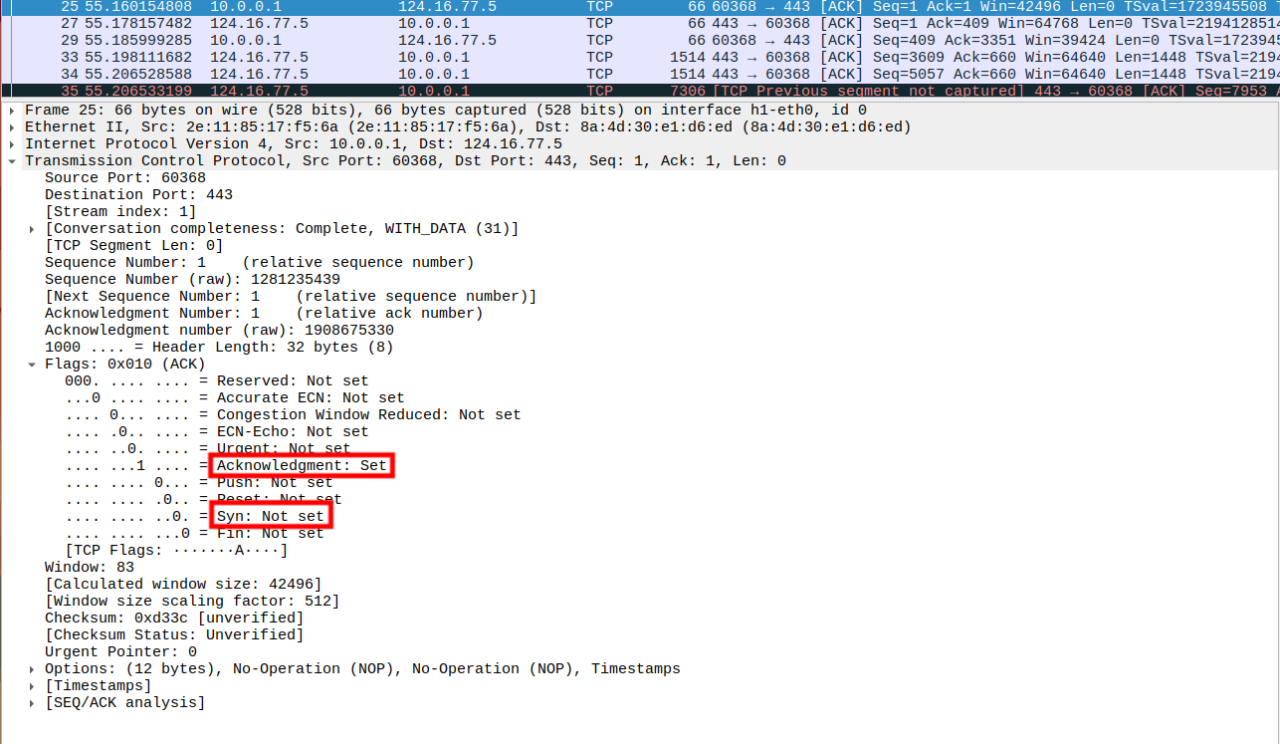
\includegraphics[width=0.8\textwidth]{fig/hand3.png}
    \caption{第三次握手}
    \label{fig:3}
  \end{figure}

  经过上述的三次握手,TCP连接正式建立,双方都置为ACK flag,交换并确认了对方的初始序列号。

  
3. 发送和收取数据(本地主机和目的主机开始HTTP访问)

  1)本地主机向域名发出GET方法报文(HTTP请求);

  2)该GET方法报文通过TCP->IP(DNS) ->MAC (ARP)->网关->目的主机;

  3)目的主机收到数据帧,通过IP->TCP->HTTP,HTTP协议单元会回应HTTP协议格式封装好的HTML形式数据(HTTP响应)﹔从请求信息中获得客户机想访问的主机名。从请求信息中获取客户机想要访问的web资源,用读取到的web资源数据,创建一个HTTP响应。
  
  4)该HTML数据通过TCP->IP(DNS) ->MAC(ARP)->网关->我的主机;

  5)我的主机收到数据帧,通过IP->TCP->HTTP->浏览器,浏览器以网页形式显示HTML内容。

4. 四次挥手断开TCP连接




\section{实验总结}
本次实验主要是简单的动手操作,通过抓包工具wireshark抓取h1下载网页的过程,分析了ARP、DNS、TCP、HTTP等协议的运行机制。实验本身难度不大,但涉及到各种协议,需要花时间调研。通过本次实验,我对互联网协议有了更深入的了解,对网络通信的过程有了更清晰的认识。

\newpage

\begin{center}
  \LARGE \bf 实验二:流完成时间实验
\end{center}

\setcounter{section}{0}

\section{实验内容}

\begin{enumerate}

  \item 利用fct_exp.py脚本复现幻灯片中的图
  
  \item 调研解释图中的现象(TCP传输、慢启动机制等)
  
\end{enumerate}

\section{实验流程}

在终端中输入
在终端中输入 中启动 、 两个
在 终端输入 其中
分别设置为1,10, 进行不同大小的实验
在 终端中输入 获取主机 上对应大小的文件
记录每次完成传输的时间和速度,每个数据点做五次实验,取均值
根据结果绘图,复现讲义上的图

\begin{enumerate}
  \item 在fct_exp.py文件中设置好带宽和延迟参数值
  \item 在终端中输入 sudo python3 fct_exp.py
  \item 在终端中输入 xterm h1 h2启动两个host
  \item 在h2终端中输入dd if=/dev/zero of=1MB.dat bs=1M count=1,其中bs可以分别设置为1,10,100,进行不同大小的实验
  \item 在h1终端中输入wget http://10.0.0.2/1MB.dat获取主机h2上对应大小的文件
  \item 记录每次完成传输的时间和速度,每个数据点做五次实验,取均值
  \item 根据结果绘图,复现讲义上的图
\end{enumerate}


\section{实验流程}

\begin{enumerate}
  \item 对于查看不同条件下的流完成时间而言,首先在fctexp.py文件中设置好带宽和延迟参数值,然后对于不同文件大小,每个数据点重复测试5次,取平均值并记录
  
  \item 依然是根据给定的参数值,在每个数据点重复测试5次,取均值并绘图。
\end{enumerate}


\section{实验数据}

\newpage 

\textbf{10ms延迟下,带宽为10Mbps下,不同文件大小的流完成时间}

1. 文件大小为10MB

% Table generated by Excel2LaTeX from sheet 'Sheet1'
\begin{table}[htbp]
  \centering
  \caption{10MB, 10ms, 10Mbps}
    \begin{tabular}{|l|r|r|}
    \hline
    测试次数 & 流完成时间(单位s) & 传输速率(单位MB/s) \\
    \hline
    1     & 8.8   & 1.14 \\
    \hline
    2     & 8.8   & 1.14 \\
    \hline
    3     & 8.8   & 1.14 \\
    \hline
    4     & 8.8   & 1.14 \\
    \hline
    5     & 8.8   & 1.14 \\
    \hline
    均值   & 8.8   & 1.14 \\
    \hline
    \end{tabular}%
\end{table}%

2. 文件大小为100MB


% Table generated by Excel2LaTeX from sheet 'Sheet1'
\begin{table}[htbp]
  \centering
  \caption{100MB, 10ms, 10Mbps}
    \begin{tabular}{|l|r|r|}
    \hline
    序号    & \multicolumn{1}{l|}{流完成时间(单位s)} & \multicolumn{1}{l|}{传输速率(单位MB/s)} \bigstrut\\
    \hline
    \multicolumn{1}{|r|}{1} & 88    & 1.14 \bigstrut\\
    \hline
    \multicolumn{1}{|r|}{2} & 88    & 1.14 \bigstrut\\
    \hline
    \multicolumn{1}{|r|}{3} & 88    & 1.14 \bigstrut\\
    \hline
    \multicolumn{1}{|r|}{4} & 88    & 1.14 \bigstrut\\
    \hline
    \multicolumn{1}{|r|}{5} & 88    & 1.14 \bigstrut\\
    \hline
    均值    & 88    & 1.14 \bigstrut\\
    \hline
  \end{tabular}%

\end{table}%


\textbf{10ms延迟下,带宽为100Mbps下,不同文件大小的流完成时间}

1. 文件大小为10MB
% Table generated by Excel2LaTeX from sheet 'Sheet1'
\begin{table}[htbp]
  \centering
  \caption{10MB, 10ms, 100Mbps}
    \begin{tabular}{|l|r|r|}
    \hline
    序号    & \multicolumn{1}{l|}{流完成时间(单位s)} & \multicolumn{1}{l|}{传输速率(单位MB/s)} \bigstrut\\
    \hline
    \multicolumn{1}{|r|}{1} & 0.9   & 10.6 \bigstrut\\
    \hline
    \multicolumn{1}{|r|}{2} & 0.9   & 10.6 \bigstrut\\
    \hline
    \multicolumn{1}{|r|}{3} & 0.9   & 10.6 \bigstrut\\
    \hline
    \multicolumn{1}{|r|}{4} & 0.9   & 10.6 \bigstrut\\
    \hline
    \multicolumn{1}{|r|}{5} & 0.9   & 10.6 \bigstrut\\
    \hline
    均值    & 0.9   & 10.6 \bigstrut\\
    \hline
    \end{tabular}%
\end{table}%

\newpage

2. 文件大小为100MB

% Table generated by Excel2LaTeX from sheet 'Sheet1'
\begin{table}[htbp]
  \centering
  \caption{100MB, 10ms, 100Mbps}
    \begin{tabular}{|l|r|r|}
    \hline
    序号    & \multicolumn{1}{l|}{流完成时间(单位s)} & \multicolumn{1}{l|}{传输速率(单位MB/s)} \bigstrut\\
    \hline
    \multicolumn{1}{|r|}{1} & 8.8   & 11.3 \bigstrut\\
    \hline
    \multicolumn{1}{|r|}{2} & 8.8   & 11.3 \bigstrut\\
    \hline
    \multicolumn{1}{|r|}{3} & 8.8   & 11.3 \bigstrut\\
    \hline
    \multicolumn{1}{|r|}{4} & 8.8   & 11.3 \bigstrut\\
    \hline
    \multicolumn{1}{|r|}{5} & 8.8   & 11.3 \bigstrut\\
    \hline
    均值    & 8.8   & 11.3 \bigstrut\\
    \hline
    \end{tabular}%
  
\end{table}%



\textbf{10ms延迟下,带宽为1Gbps下,不同文件大小的流完成时间}

1. 文件大小为10MB
% Table generated by Excel2LaTeX from sheet 'Sheet1'
\begin{table}[htbp]
  \centering
  \caption{10MB, 10ms, 1Gbps}
    \begin{tabular}{|l|r|r|}
    \hline
    序号    & \multicolumn{1}{l|}{流完成时间(单位s)} & \multicolumn{1}{l|}{传输速率(单位MB/s)} \bigstrut\\
    \hline
    \multicolumn{1}{|r|}{1} & 0.2   & 46 \bigstrut\\
    \hline
    \multicolumn{1}{|r|}{2} & 0.2   & 45.9 \bigstrut\\
    \hline
    \multicolumn{1}{|r|}{3} & 0.2   & 46.1 \bigstrut\\
    \hline
    \multicolumn{1}{|r|}{4} & 0.2   & 46 \bigstrut\\
    \hline
    \multicolumn{1}{|r|}{5} & 0.2   & 46 \bigstrut\\
    \hline
    均值    & 0.2   & 46 \bigstrut\\
    \hline
    \end{tabular}%
  
\end{table}%




2. 文件大小为100MB

% Table generated by Excel2LaTeX from sheet 'Sheet1'
\begin{table}[htbp]
  \centering
  \caption{100MB, 10ms, 1Gbps}
    \begin{tabular}{|l|r|r|}
    \hline
    序号    & \multicolumn{1}{l|}{流完成时间(单位s)} & \multicolumn{1}{l|}{传输速率(单位MB/s)} \bigstrut\\
    \hline
    \multicolumn{1}{|r|}{1} & 1     & 98.7 \bigstrut\\
    \hline
    \multicolumn{1}{|r|}{2} & 1     & 98.9 \bigstrut\\
    \hline
    \multicolumn{1}{|r|}{3} & 1     & 99.3 \bigstrut\\
    \hline
    \multicolumn{1}{|r|}{4} & 1     & 99.2 \bigstrut\\
    \hline
    \multicolumn{1}{|r|}{5} & 1     & 99.3 \bigstrut\\
    \hline
    均值    & 1     & 99.08 \bigstrut\\
    \hline
    \end{tabular}%
  
\end{table}%

\newpage


\textbf{100ms延迟下,带宽为10Mbps下,不同文件大小的流完成时间}

1. 文件大小为10MB

% Table generated by Excel2LaTeX from sheet 'Sheet1'
\begin{table}[htbp]
  \centering
  \caption{10MB, 100ms, 10Mbps}
    \begin{tabular}{|l|r|r|}
    \hline
    序号    & \multicolumn{1}{l|}{流完成时间(单位s)} & \multicolumn{1}{l|}{传输速率(单位MB/s)} \bigstrut\\
    \hline
    \multicolumn{1}{|r|}{1} & 9.4   & 1.14 \bigstrut\\
    \hline
    \multicolumn{1}{|r|}{2} & 9.4   & 1.14 \bigstrut\\
    \hline
    \multicolumn{1}{|r|}{3} & 9.4   & 1.14 \bigstrut\\
    \hline
    \multicolumn{1}{|r|}{4} & 9.4   & 1.14 \bigstrut\\
    \hline
    \multicolumn{1}{|r|}{5} & 9.4   & 1.14 \bigstrut\\
    \hline
    均值    & 9.4   & 1.14 \bigstrut\\
    \hline
    \end{tabular}%
  
\end{table}%


2. 文件大小为100MB

% Table generated by Excel2LaTeX from sheet 'Sheet1'
\begin{table}[htbp]
  \centering
  \caption{100MB, 100ms, 10Mbps}
    \begin{tabular}{|l|r|r|}
    \hline
    序号    & \multicolumn{1}{l|}{流完成时间(单位s)} & \multicolumn{1}{l|}{传输速率(单位MB/s)} \bigstrut\\
    \hline
    \multicolumn{1}{|r|}{1} & 88    & 1.14 \bigstrut\\
    \hline
    \multicolumn{1}{|r|}{2} & 88    & 1.14 \bigstrut\\
    \hline
    \multicolumn{1}{|r|}{3} & 88    & 1.14 \bigstrut\\
    \hline
    \multicolumn{1}{|r|}{4} & 88    & 1.14 \bigstrut\\
    \hline
    \multicolumn{1}{|r|}{5} & 88    & 1.14 \bigstrut\\
    \hline
    均值    & 88    & 1.14 \bigstrut\\
    \hline
    \end{tabular}%
  
\end{table}%


\textbf{100ms延迟下,带宽为100Mbps下,不同文件大小的流完成时间}

1. 文件大小为10MB

% Table generated by Excel2LaTeX from sheet 'Sheet1'
\begin{table}[htbp]
  \centering
  \caption{10MB, 100ms, 100Mbps}
    \begin{tabular}{|l|r|r|}
    \hline
    序号    & \multicolumn{1}{l|}{流完成时间(单位s)} & \multicolumn{1}{l|}{传输速率(单位MB/s)} \bigstrut\\
    \hline
    \multicolumn{1}{|r|}{1} & 2.3   & 4.28 \bigstrut\\
    \hline
    \multicolumn{1}{|r|}{2} & 2.3   & 4.28 \bigstrut\\
    \hline
    \multicolumn{1}{|r|}{3} & 2.3   & 4.28 \bigstrut\\
    \hline
    \multicolumn{1}{|r|}{4} & 2.3   & 4.28 \bigstrut\\
    \hline
    \multicolumn{1}{|r|}{5} & 2.3   & 4.28 \bigstrut\\
    \hline
    均值    & 2.3   & 4.28 \bigstrut\\
    \hline
    \end{tabular}%
  
\end{table}%

\newpage 

2. 文件大小为100MB

% Table generated by Excel2LaTeX from sheet 'Sheet1'
\begin{table}[htbp]
  \centering
  \caption{100MB, 100ms, 100Mbps}
    \begin{tabular}{|l|r|r|}
    \hline
    序号    & \multicolumn{1}{l|}{流完成时间(单位s)} & \multicolumn{1}{l|}{传输速率(单位MB/s)} \bigstrut\\
    \hline
    \multicolumn{1}{|r|}{1} & 10    & 11.4 \bigstrut\\
    \hline
    \multicolumn{1}{|r|}{2} & 10    & 11.4 \bigstrut\\
    \hline
    \multicolumn{1}{|r|}{3} & 10    & 11.4 \bigstrut\\
    \hline
    \multicolumn{1}{|r|}{4} & 10    & 11.4 \bigstrut\\
    \hline
    \multicolumn{1}{|r|}{5} & 10    & 11.4 \bigstrut\\
    \hline
    均值    & 10    & 11.4 \bigstrut\\
    \hline
    \end{tabular}%
  
\end{table}%



\textbf{100ms延迟下,带宽为1Gbps下,不同文件大小的流完成时间}

1. 文件大小为10MB

% Table generated by Excel2LaTeX from sheet 'Sheet1'
\begin{table}[htbp]
  \centering
  \caption{10MB, 100ms, 1Gbps}
    \begin{tabular}{|l|r|r|}
    \hline
    序号    & \multicolumn{1}{l|}{流完成时间(单位s)} & \multicolumn{1}{l|}{传输速率(单位MB/s)} \bigstrut\\
    \hline
    \multicolumn{1}{|r|}{1} & 1.8   & 5.47 \bigstrut\\
    \hline
    \multicolumn{1}{|r|}{2} & 2     & 4.99 \bigstrut\\
    \hline
    \multicolumn{1}{|r|}{3} & 1.8   & 5.45 \bigstrut\\
    \hline
    \multicolumn{1}{|r|}{4} & 1.8   & 5.47 \bigstrut\\
    \hline
    \multicolumn{1}{|r|}{5} & 1.8   & 5.47 \bigstrut\\
    \hline
    均值    & 1.84  & 5.37 \bigstrut\\
    \hline
    \end{tabular}%
  
\end{table}%


2. 文件大小为100MB


% Table generated by Excel2LaTeX from sheet 'Sheet1'
\begin{table}[htbp]
  \centering
  \caption{100MB, 100ms, 1Gbps}
    \begin{tabular}{|l|r|r|}
    \hline
    序号    & \multicolumn{1}{l|}{流完成时间(单位s)} & \multicolumn{1}{l|}{传输速率(单位MB/s)} \bigstrut\\
    \hline
    \multicolumn{1}{|r|}{1} & 3.5   & 28.5 \bigstrut\\
    \hline
    \multicolumn{1}{|r|}{2} & 3.5   & 28.5 \bigstrut\\
    \hline
    \multicolumn{1}{|r|}{3} & 3.5   & 28.5 \bigstrut\\
    \hline
    \multicolumn{1}{|r|}{4} & 3.5   & 28.5 \bigstrut\\
    \hline
    \multicolumn{1}{|r|}{5} & 3.5   & 28.5 \bigstrut\\
    \hline
    均值    & 3.5   & 28.5 \bigstrut\\
    \hline
    \end{tabular}%
  
\end{table}%


\newpage



% Table generated by Excel2LaTeX from sheet 'Sheet1'
\textbf{下面是复现讲义图而做的不同带宽和数据包大小的实验,其中流完成时间单位为s, 传输速率单位为MB/s}
\begin{table}[htbp]
  \centering
  \caption{复现讲义图过程测量数据}
    \begin{tabular}{|c|l|r|r|r|r|r|r|r|r|r|r|}
    \hline
          &       & \multicolumn{1}{l|}{时间} & \multicolumn{1}{l|}{传输速率} & \multicolumn{1}{l|}{时间} & \multicolumn{1}{l|}{传输速率} & \multicolumn{1}{l|}{时间} & \multicolumn{1}{l|}{传输速率} & \multicolumn{1}{l|}{时间} & \multicolumn{1}{l|}{传输速率} & \multicolumn{1}{l|}{时间} & \multicolumn{1}{l|}{传输速率} \bigstrut\\
    \hline
          & 序号    & \multicolumn{2}{c|}{10Mbps} & \multicolumn{2}{c|}{50Mbps} & \multicolumn{2}{c|}{100Mbps} & \multicolumn{2}{c|}{500Mbps} & \multicolumn{2}{c|}{1Gbps} \bigstrut\\
    \hline
    \multirow{6}[12]{*}{1MB} & \multicolumn{1}{r|}{1} & 1.5   & 675   & 1.2   & 837   & 1.2   & 845   & 1.2   & 851   & 1.2   & 851 \bigstrut\\
\cline{2-12}          & \multicolumn{1}{r|}{2} & 1.5   & 675   & 1.2   & 837   & 1.2   & 845   & 1.2   & 849   & 1.2   & 851 \bigstrut\\
\cline{2-12}          & \multicolumn{1}{r|}{3} & 1.5   & 675   & 1.2   & 837   & 1.2   & 845   & 1.2   & 852   & 1.2   & 849 \bigstrut\\
\cline{2-12}          & \multicolumn{1}{r|}{4} & 1.5   & 675   & 1.2   & 837   & 1.2   & 845   & 1.2   & 851   & 1.2   & 851 \bigstrut\\
\cline{2-12}          & \multicolumn{1}{r|}{5} & 1.5   & 675   & 1.2   & 837   & 1.2   & 845   & 1.2   & 848   & 1.2   & 852 \bigstrut\\
\cline{2-12}          & 均值    & 1.5   & 675   & 1.2   & 837   & 1.2   & 845   & 1.2   & 850.2 & 1.2   & 850.8 \bigstrut\\
    \hline
    \multirow{6}[12]{*}{10MB} & \multicolumn{1}{r|}{1} & 9.4   & 1.14  & 3.1   & 3.22  & 2.3   & 4.28  & 1.9   & 5.4   & 1.8   & 5.47 \bigstrut\\
\cline{2-12}          & \multicolumn{1}{r|}{2} & 9.4   & 1.14  & 3.1   & 3.22  & 2.3   & 4.28  & 1.9   & 5.4   & 2     & 4.99 \bigstrut\\
\cline{2-12}          & \multicolumn{1}{r|}{3} & 9.4   & 1.14  & 3.1   & 3.22  & 2.3   & 4.28  & 1.9   & 5.4   & 1.8   & 5.45 \bigstrut\\
\cline{2-12}          & \multicolumn{1}{r|}{4} & 9.4   & 1.14  & 3.1   & 3.22  & 2.3   & 4.28  & 1.9   & 5.4   & 1.8   & 5.47 \bigstrut\\
\cline{2-12}          & \multicolumn{1}{r|}{5} & 9.4   & 1.14  & 3.1   & 3.22  & 2.3   & 4.28  & 1.9   & 5.4   & 1.8   & 5.47 \bigstrut\\
\cline{2-12}          & 均值    & 9.4   & 1.14  & 3.1   & 3.22  & 2.3   & 4.28  & 1.9   & 5.4   & 1.84  & 5.37 \bigstrut\\
    \hline
    \multirow{6}[12]{*}{100MB} & \multicolumn{1}{r|}{1} & 88    & 1.14  & 19    & 5.7   & 10    & 11.4  & 4.1   & 25.7  & 3.5   & 28.5 \bigstrut\\
\cline{2-12}          & \multicolumn{1}{r|}{2} & 88    & 1.14  & 19    & 5.7   & 10    & 11.4  & 4.2   & 26.6  & 3.5   & 28.5 \bigstrut\\
\cline{2-12}          & \multicolumn{1}{r|}{3} & 88    & 1.14  & 19    & 5.7   & 10    & 11.4  & 3.7   & 27.4  & 3.5   & 28.5 \bigstrut\\
\cline{2-12}          & \multicolumn{1}{r|}{4} & 88    & 1.14  & 19    & 5.7   & 10    & 11.4  & 4.1   & 26.9  & 3.5   & 28.5 \bigstrut\\
\cline{2-12}          & \multicolumn{1}{r|}{5} & 88    & 1.14  & 19    & 5.7   & 10    & 11.4  & 4.1   & 25.7  & 3.5   & 28.5 \bigstrut\\
\cline{2-12}          & 均值    & 88    & 1.14  & 19    & 5.7   & 10    & 11.4  & 4.04  & 26.46 & 3.5   & 28.5 \bigstrut\\
    \hline
    \end{tabular}%
\end{table}%

\newpage


通过软件绘图后,得到如下图像:

\begin{figure}[!htbp]
  \centering
  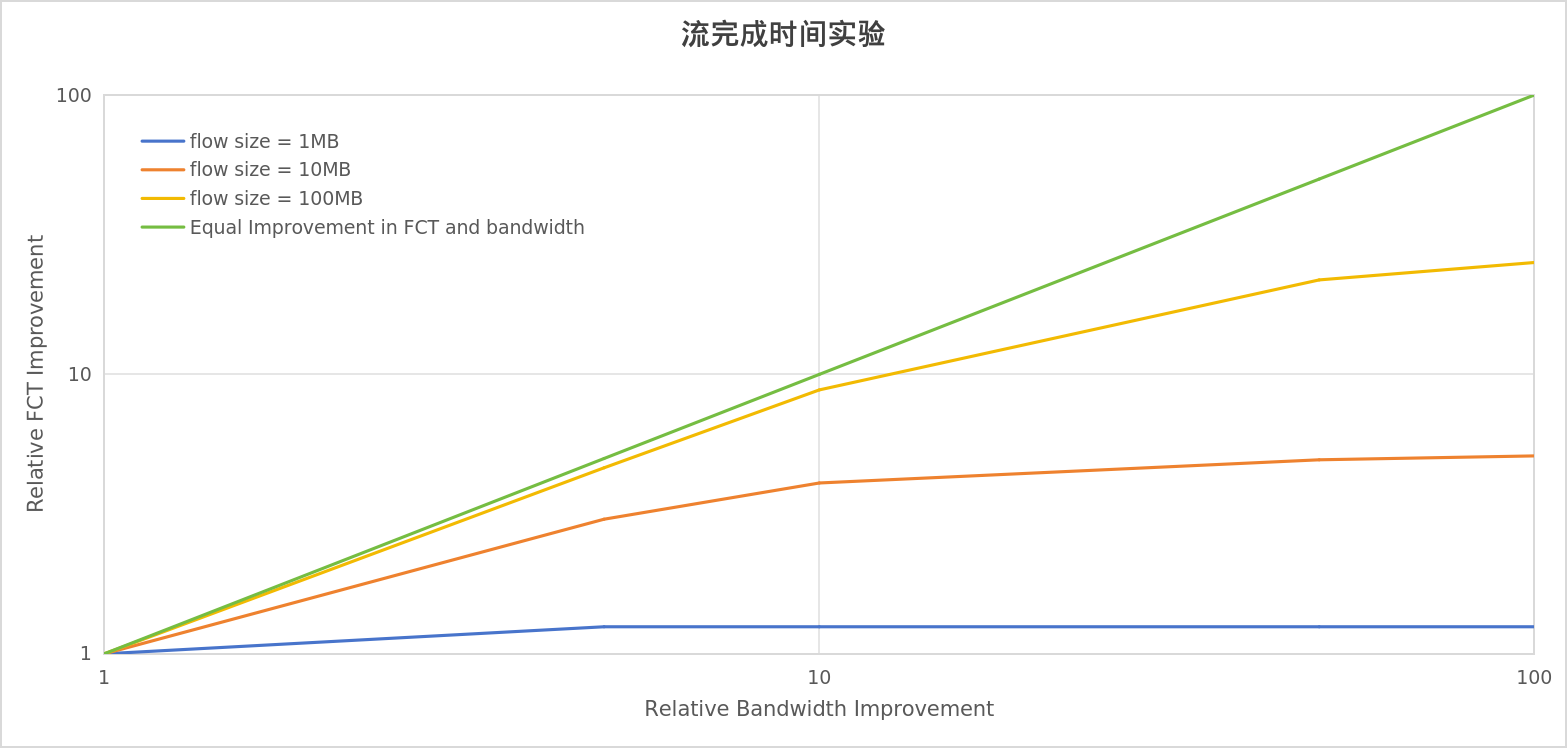
\includegraphics[width=0.8\textwidth]{fig/output.png}
  \caption{流完成时间}
\end{figure}

可以看到绘制图像与讲义中的图像基本一致,复现效果良好。

\vspace{2em}

对图中现象及实验结果的现象进行总结:
\begin{enumerate}
  \item 在带宽一定时,传输速率与数据包大小成正比
  \item 在数据包大小一定时,传输速率并不会随着带宽线性增加(传输速率的增加速度随带宽增加变缓)。对于各个大小的数据包而言,当带宽达到500Mbps后,传输速率基本不再增加
  \item 当带宽达到50Mbps后, 1MB数据包的传输速率不再因为带宽改变而发生改变
  \item 在改变延迟的实验中发现,减小延迟可以显著增加高带宽、大数据包的传输速率。同时在实验过程中也可以较为明显的观察到,在数据包开始传输的一段时间内速度是较慢的,有一个逐步增加的过程。这段时间的长短与延迟成正相关,100ms延迟下时间较长,10ms延迟下时间较短。
\end{enumerate}


\section{拓展调研}


\textbf{TCP传输}

TCP协议会将应用层的数据流分割成适当长度的报文段,最大传输段大小(MSS) 通常受该计算机连接的网络的数据链路层的最大传送单元(MTU)限制。而TCP的传输速率是由其阻塞算法决定的,TCP拥塞算法缓慢地探测网络的可用带宽 增加传输速率直到检测到分组丢失,然后指数地降低传输速率。

当数据包大小不变带宽增加时 该算法会增加传输速率直至分组丢失 而降低传输速率时指数级的 因此速率并不会随着带宽的增加而线性增加。

同时 对数据进行分组也会造成丢包、排队、阻塞等问题 这也会影响到传输速率的增长。


\vspace{2em}
\textbf{慢启动机制}

慢启动是TCP使用的一种阻塞控制机制。慢启动也叫做指数增长期。慢启动是指每次TCP接收窗口收到确认时都会增长。增加的大小就是已确认段的数目。这种情况一直保持到要么没有收到一些段 要么窗口大小到达预先定义的阈值。如果发生丢失事件 TCP就认为这是网络阻塞 就会采取措施减轻网络拥挤。一旦发生丢失事件或者到达阈值 TCP就会进入线性增长阶段。这时,每经过一个RTT窗口增长一个段。

由于TCP连接会随着时间进行自我调谐,起初会限制连接的最大速度,如果数据传输成功,会随着时间的推移提高传输速度。这就是TCP的慢启动机制。

这样就解释了在带宽较高时,小数据包没有达到期待的网速的问题。在慢启动阶段TCP预的窗口大小会随着每接受到一个段而指数级增长,对于数据包大小较小的包,在窗口还没有达到带宽的阈值时可能传输就已经结束了,因此此时测得的传输速率会明显小于对应带宽的最大速率。

\section{实验总结}

\begin{enumerate}
  \item 本次实验通过对不同带宽、延迟、数据包大小的传输过程进行定量测量,给我带来了更加直观的印象,可以更好地理解网络传输的机制,对于网络的性能优化有一定的帮助。
  \item 此外,通过调研,也加深了我对TCP协议的认识,对于网络传输的机制有了更深入的了解。
  \item 通过复现讲义的效果图并分析,我也对影响网速的因素有了进一步的认识
\end{enumerate}









\end{document}